\documentclass{article}
\usepackage[utf8]{inputenc}
\usepackage[T1]{fontenc}
\usepackage[russian]{babel}
\usepackage{tikz}
\usepackage{graphicx}
\usepackage{titlesec}
\usepackage{amsfonts}
\usepackage{amsmath}
\usepackage{bbm}
\usepackage[left=2cm,right=2cm,
    top=2cm,bottom=2cm,bindingoffset=0cm]{geometry}
\renewcommand{\thesection}{\arabic{section}}
\titleformat{\section}{\large\bfseries}{\thesection}{1em}{}
\title{Пределы}
\author{Каренин Константин Витальевич}
\date{16.12.2023}
\begin{document}

\begin{titlepage}
    \centering
    \vspace*{0.5 cm}
    
    \textsc{\LARGE \textbf{Линейная алгебра}}
    \vspace{1.5cm}
    
    \rule{\linewidth}{0.2 mm} \\[0.4 cm]
    { \huge \bfseries Аналитическая геометрия}
    \rule{\linewidth}{0.2 mm} \\[1.5 cm]
    
    \Large Выполнили: \\
    Каренин Константин \\
    Темиров Тимур \\
    Гонин Сергей \\
    
    \vspace{0.5cm}
    
    Группа: М3104
    
    \vspace{0.5cm}
    
    Преподаватель: Сарычев Павел
    
    \vspace{0.5cm}
    
    Университет ИТМО
    
    \vfill

    
\includegraphics[height=70px]{logo.jpg}
    
    16.12.2023
    
\end{titlepage}

\setcounter{page}{2}

% task 1
\newpage
\section{В основании призмы1 $ABCDA_1B_1C_1D_1$ лежит ромб с острым углом $A = 60^\circ$.
Точка K лежит на продолжении ребра $AB$ за точку $B$, причем угол $ADK$ прямой.
Найти координаты точки пространства в системе координат $A, \overrightarrow{AB}, \overrightarrow{AD}, \overrightarrow{AA_1}$, если
известны ее координаты $x', y', z'$ в системе координат $K, \overrightarrow{KA}, \overrightarrow{KD}, \overrightarrow{KC_1}$
}
    На всех графиках точки $A_1, B_1, C_1, D_1$ подписаны как $E, F, G, H$ соответственно \\
    Тело в пространстве: \\
    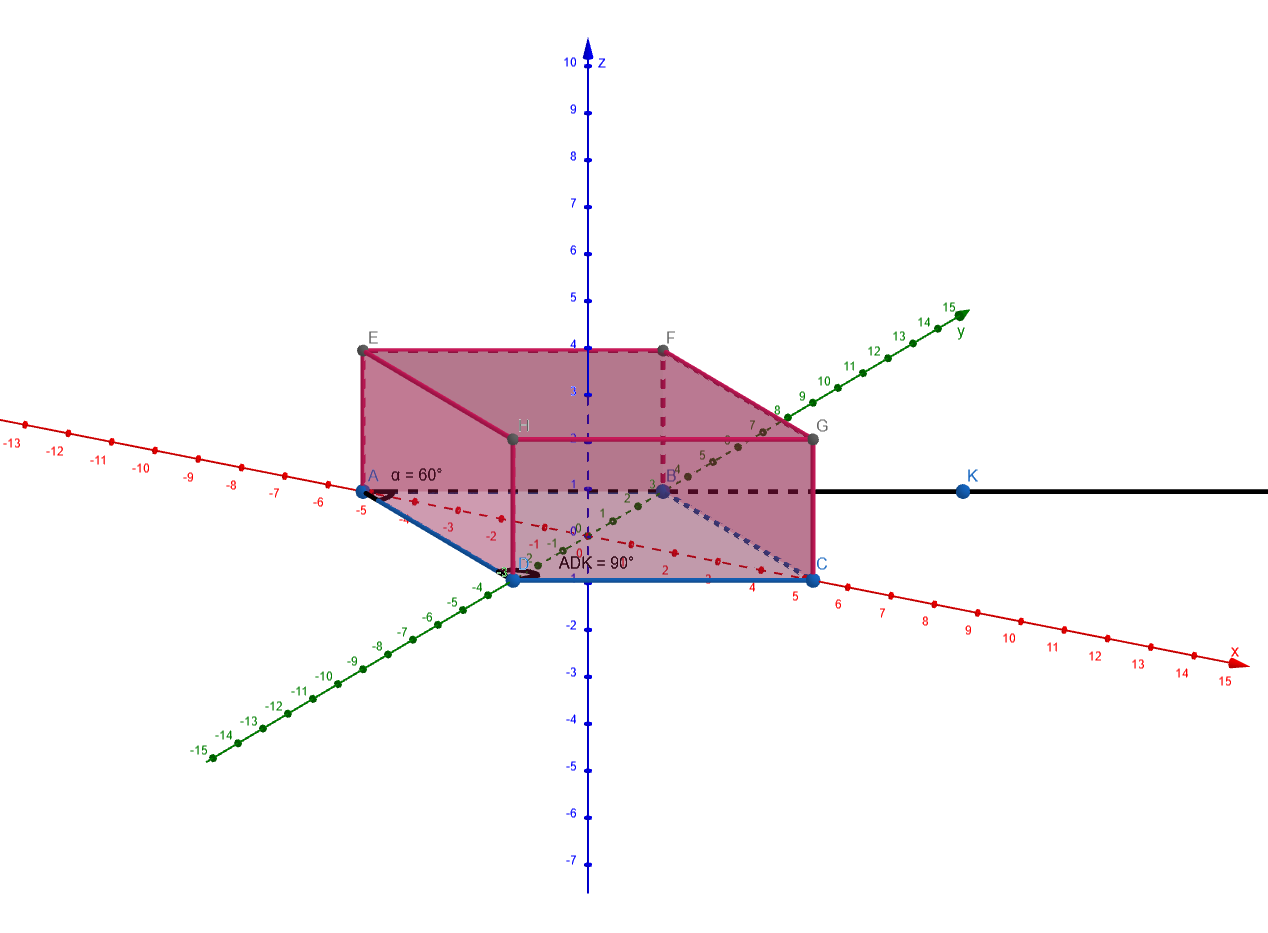
\includegraphics[height=200px]{img1.png} \\
    Система координат $A, \overrightarrow{AB}, \overrightarrow{AD}, \overrightarrow{AA_1}$: \\
    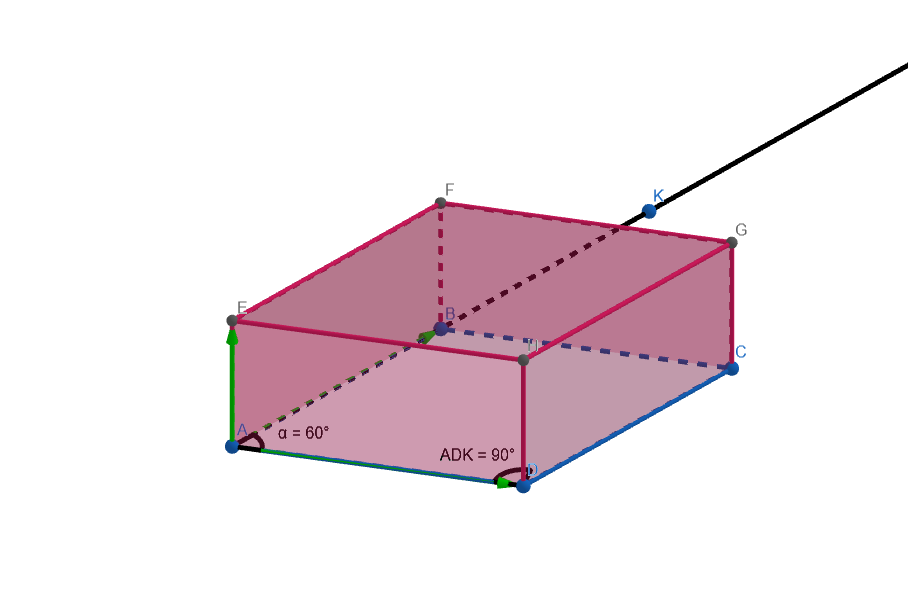
\includegraphics[height=200px]{img2.png} \\
    Система координат $K, \overrightarrow{KA}, \overrightarrow{KD}, \overrightarrow{KC_1}$: \\
    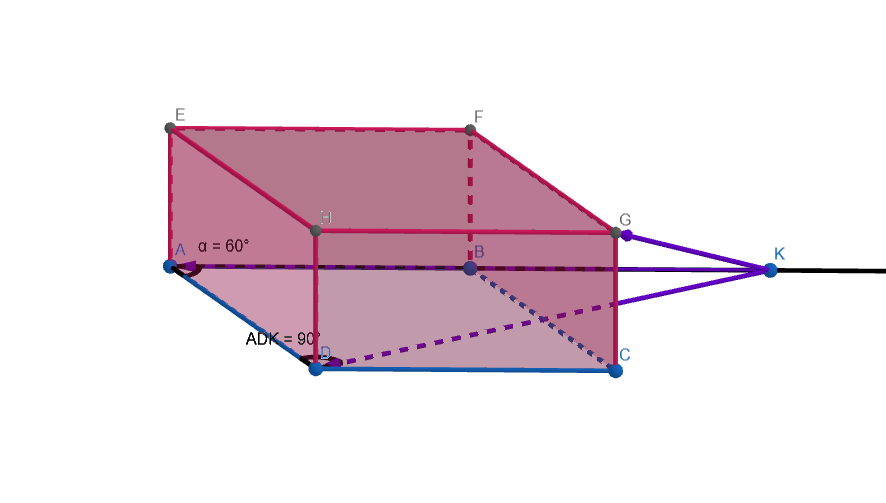
\includegraphics[height=200px]{img3.png} \\ \\ \\ \\
    Обе системы координат: \\
    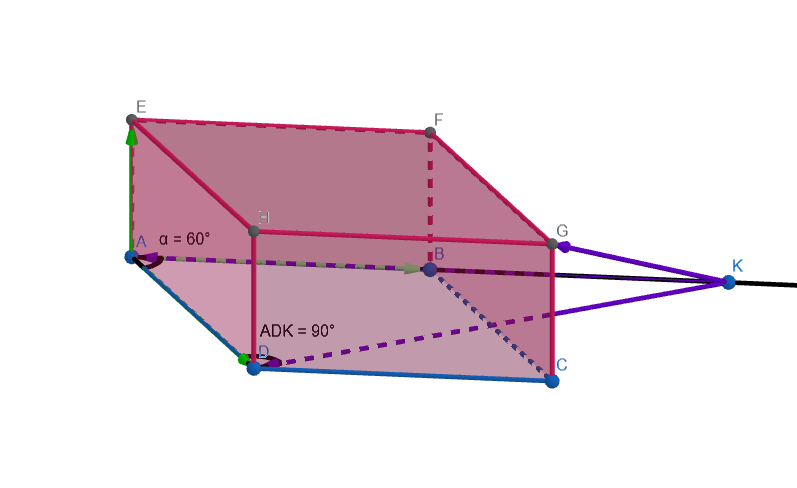
\includegraphics[height=200px]{img4.png} \\
    По теореме о катете лежащем против угла в 30 градусов следует что: \\
    $AD = \frac{1}{2} AK$ \\
    $AB + BK = AK$ \\
    $AB = AD$ \\
    $AD + BK = AK$ \\
    $BK = AK - AD = \frac{1}{2} AK$ \\
    Пусть точка $O$ имеет координы $(x', y', z')$, тогда найдем ради
    $\overrightarrow{AO} = x' \overrightarrow{AB} + y' \overrightarrow{AD} + z' \overrightarrow{AA_1}$ \\
    Выразим базисные векторы первого базиза через векторы второго \\
    \begin{equation*}
        \begin{cases}
            \overrightarrow{AB} = - \frac{1}{2} \overrightarrow{KA} \\
            \overrightarrow{AD} = \overrightarrow{KD} - \overrightarrow{KA} \\
            \overrightarrow{AA_1} = \overrightarrow{KC_1} - \overrightarrow{AB} - \overrightarrow{AD} = \overrightarrow{KC_1} - \overrightarrow{KD} + 3 \overrightarrow{KA} \\
        \end{cases}
    \end{equation*}
    $\overrightarrow{AO} = -\overrightarrow{KA} + \overrightarrow{KO}$ \\
    $\overrightarrow{KO} = \overrightarrow{AO} - \overrightarrow{KA} = -\overrightarrow{KA} + x' \overrightarrow{AB} + y' \overrightarrow{AD} + z' \overrightarrow{AA_1} = -\overrightarrow{KA} - \frac{1}{2} x' \overrightarrow{KA} + y' \overrightarrow{KD} - y' \overrightarrow{KA} - z' \overrightarrow{KC_1} + 3z' \overrightarrow{KA} = \overrightarrow{KA} (-1 - \frac{1}{2}x' - y' + 3z') + (y'-z') \overrightarrow{KD} + z' \overrightarrow{KC_1}$ \\
    $O(-1 - \frac{1}{2}x' - y' + 3z', y'-z', z')$ \\ \\
    Для проверки построим точку $X$: \\
    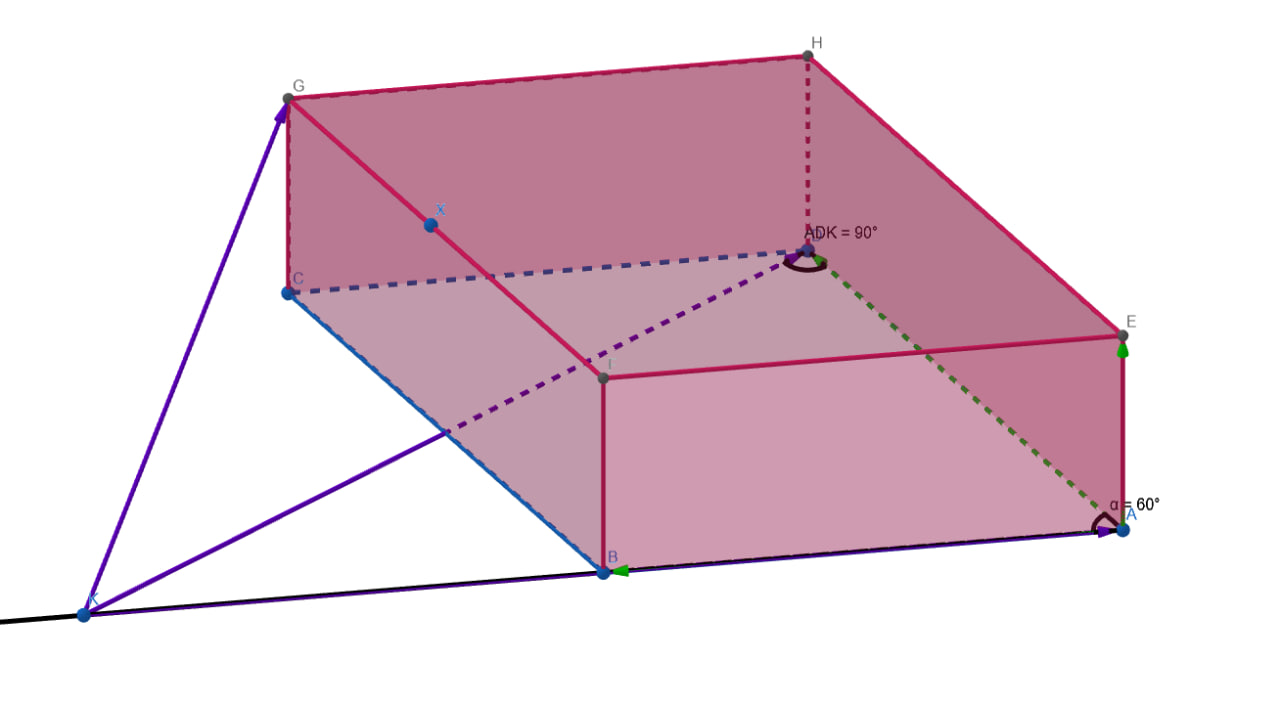
\includegraphics[height=200px]{img6.jpg} \\
    Переведя её координаты из системы координат $K, \overrightarrow{KA}, \overrightarrow{KD}, \overrightarrow{KC_1}$ в систему координат $A, \overrightarrow{AB}, \overrightarrow{AD}, \overrightarrow{AA_1}$, заметим что вычисленные координаты совпадают с реальными, значит всё верно

% task 3
\newpage
\section{Составьте уравнение геометрического места центров окружностей, проходящих
через точку $M(3,4)$ и касающихся оси абсцисс}
    Изобразим условие задачи: \\
    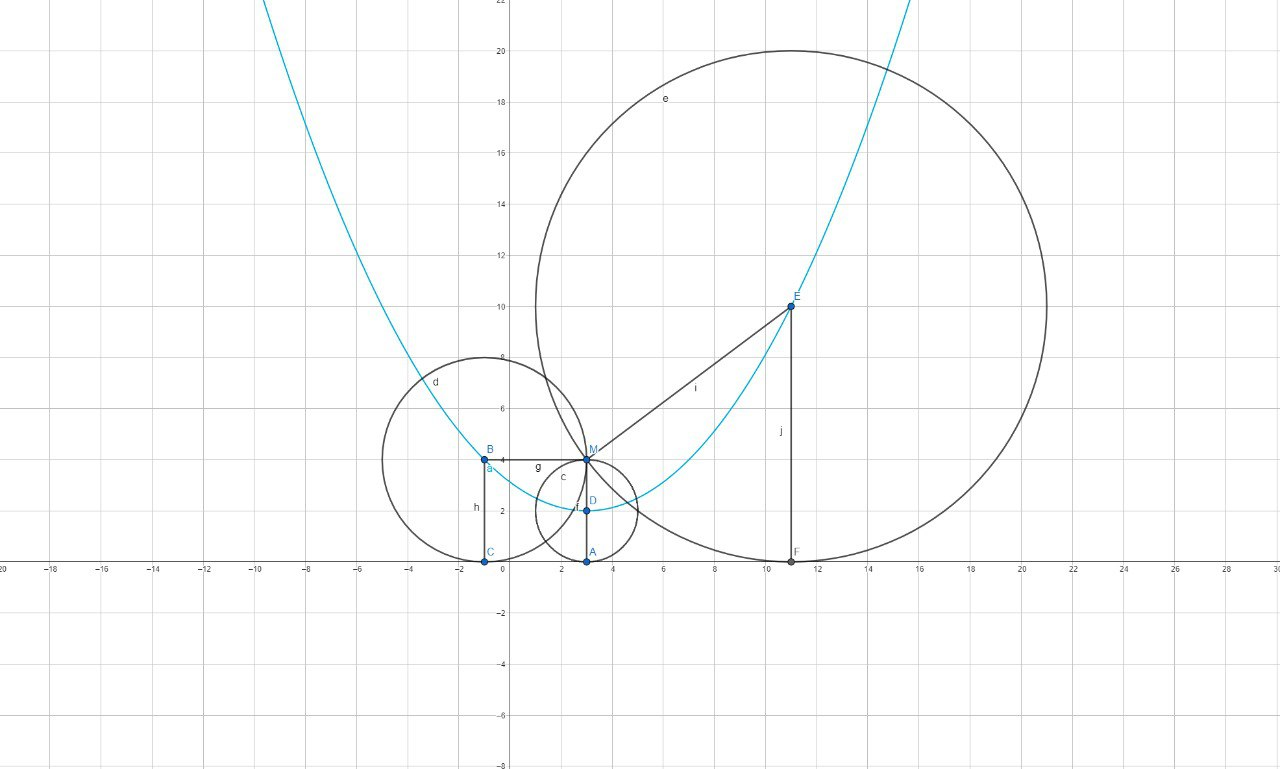
\includegraphics[height=200px]{img3_5.jpg} \\
    Радиус и центр окружности: Поскольку окружность касается оси абсцисс, ее радиус равен абсолютному значению ординаты ее центра. Пусть $C(x,y)$ - центр такой окружности. Тогда радиус $R=|y|$. \\
    Прохождение через точку $M(3,4)$: Расстояние от центра $C(x,y)$ до точки $M(3,4)$ должно быть равно радиусу окружности. Следовательно, мы можем использовать уравнение окружности для этого условия:
    $(x - 3)^2 + (y - 4)^2=R^2$ \\ \\
    Решим уравнение: \\
    $|OM| = y_0$ \\
    $\overrightarrow{OM} \{3-x_0, 4 - y_0\}$ \\
    $|OM| = \sqrt{(3 - x_0)^2 + (4 - y_0)^2}$ \\
    $|OM| = y_0^2$ \\
    $(3 - x_0)^2 + (4 - y_0)^2 = y_0^2$ \\
    $y_0 = \frac{1}{8}(3 - x_0)^2 + 2$ \\
    Изобразим множество: \\
    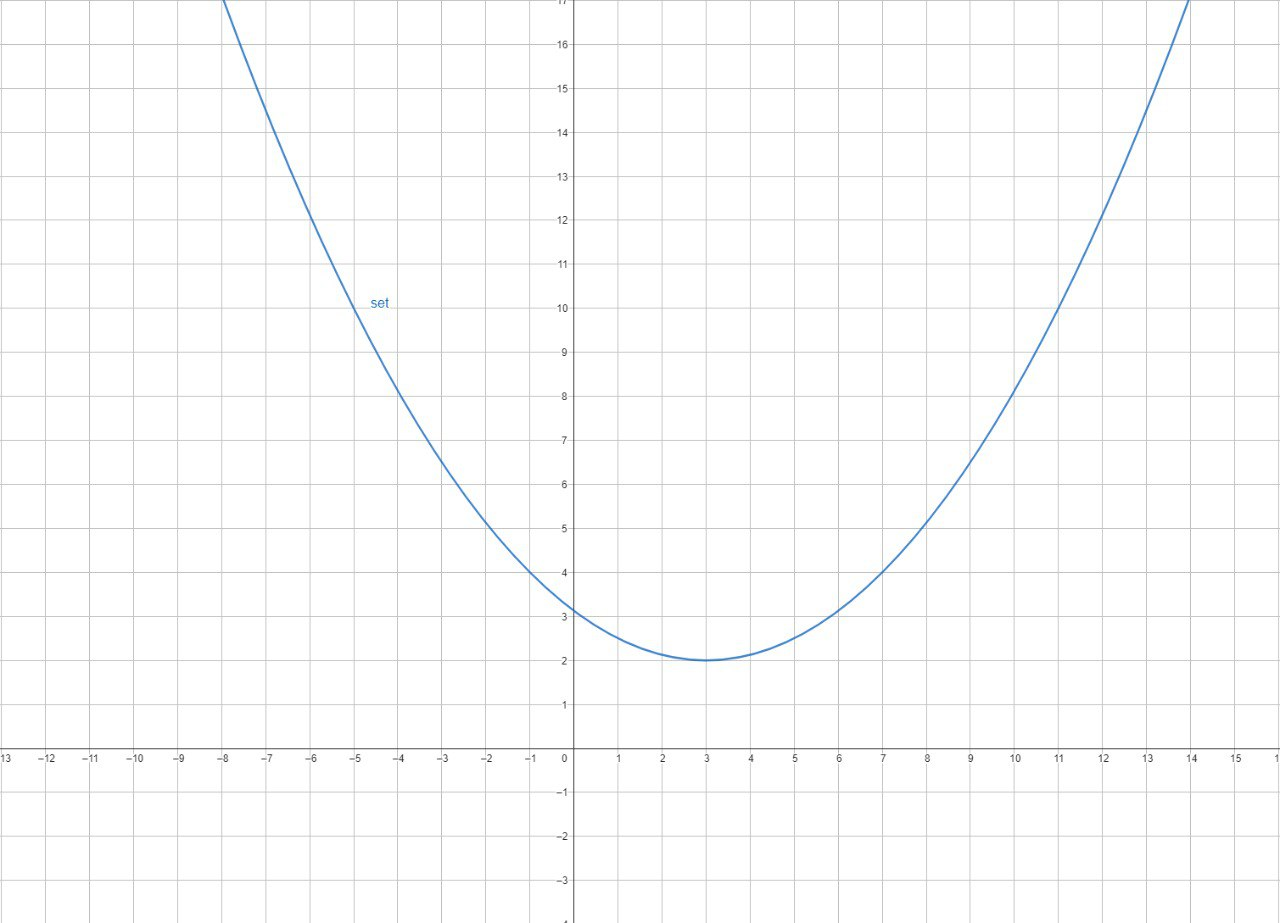
\includegraphics[height=200px]{img3_6.jpg}
    

% task 4
\newpage
\section{Даны $T_1$ и $T_2$ – тела, ограниченные поверхностями не выше второго порядка}
    \subsection{Запишите уравнения и названия поверхностей, ограничивающих тело $T_1$}
        Заметим, что фигура $T_1$ состоит из полуокружности, двух параллельных прямых и наклонной прямой. Значит $T_1$ ограничена цилиндром, шаром и двухполосным гиперболоидом.
        \begin{equation*} 
        \begin{cases}
            \frac{1}{4}(y + 6)^2 = x^2 + (z + 1)^2 \text{ - двуполосный гиперболоид}\\ 
            \begin{cases}
                x^2 + z^2 = 1 \\
                y < 0 \\
            \end{cases} \text{ - цилиндр элементарный} \\
            \begin{cases}
                x^2 + y^2 + z^2 = 1 \\
                y \geq 0 \\
            \end{cases} \text{ - шар} \\
        \end{cases}
        \end{equation*}
    \subsection{Изобразите тело $T_2$ и его проекции на координатные плоскости}
        Изображение в 3х плоскостях: \\
        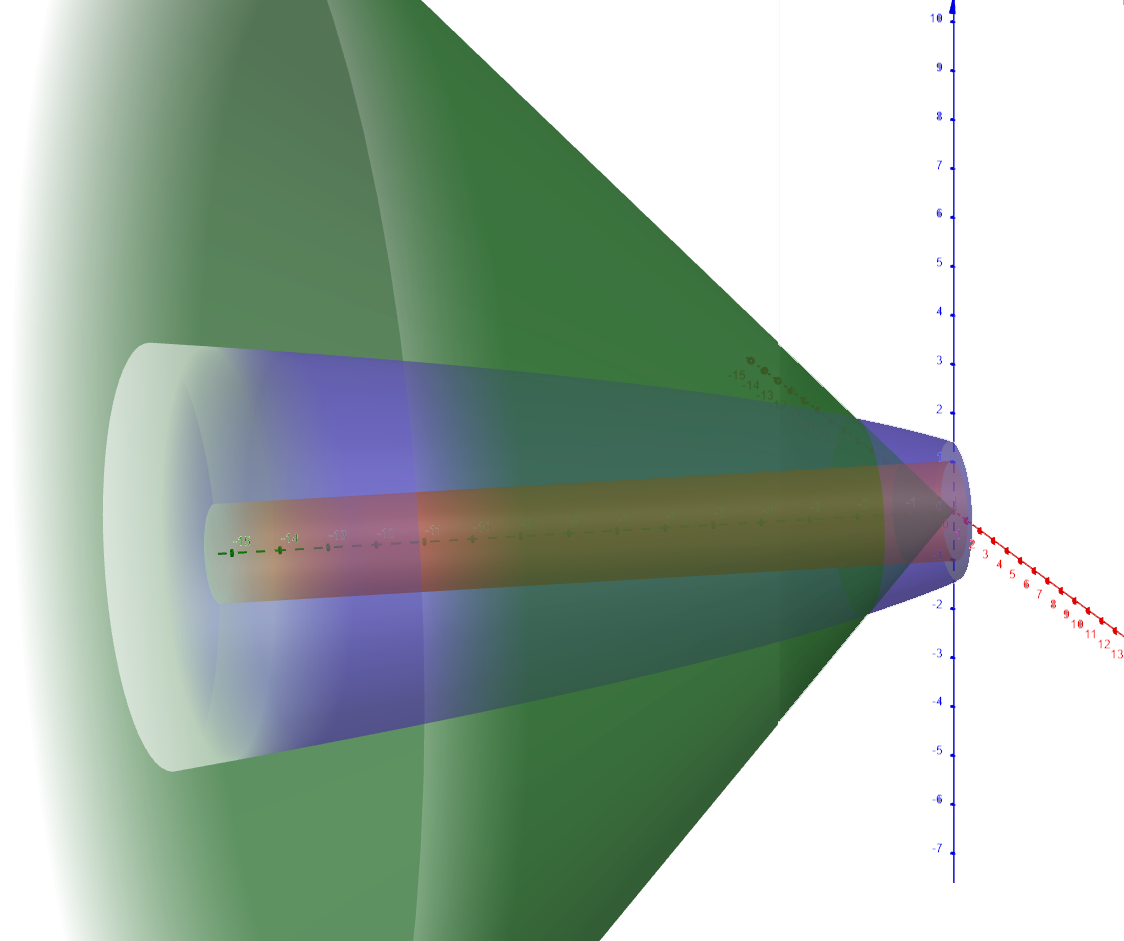
\includegraphics[height=200px]{img4_1.png} \\
        Проекция на $O_{xz}$: \\
        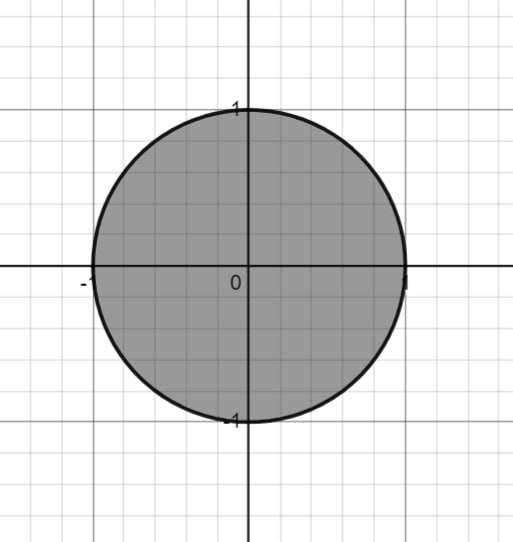
\includegraphics[height=200px]{xy.jpg} \\ \\ \\ \\ \\ \\
        Проекция на $O_{yz}$: \\
        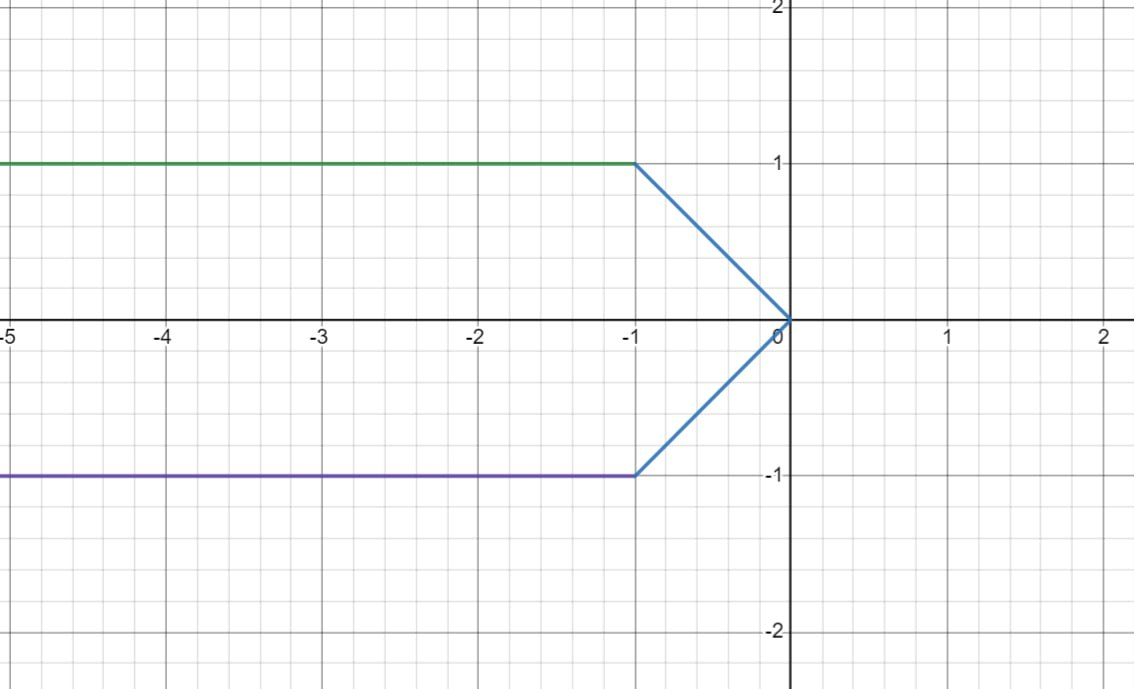
\includegraphics[height=200px]{zx.jpg} \\
        Проекция на $O_{yx}$: \\
        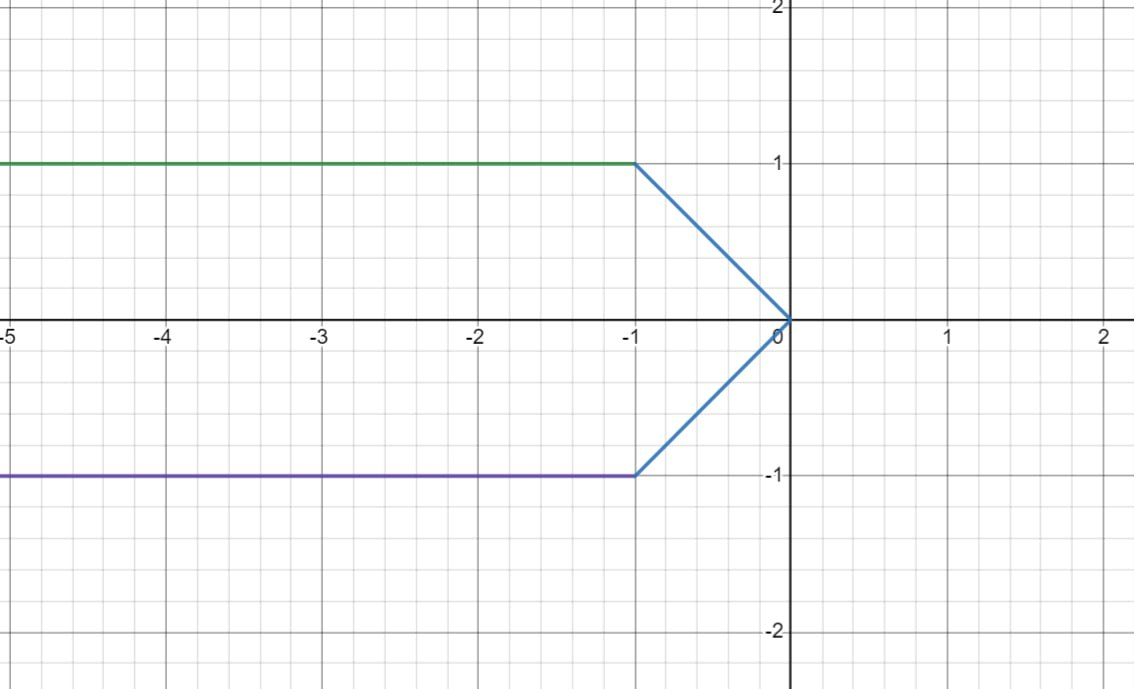
\includegraphics[height=200px]{zy.jpg} \\
    
    
% evaluation paper
\newpage
\[
\renewcommand{\arraystretch}{2}
\begin{tabular}{| c | c |}
 \hline
    \hugeУчастник & \hugeВклад в \% \\
 \hline
    \hugeКаренин Константин & \huge33.(3) \\
 \hline
    \hugeГонин Сергей & \huge33.(3) \\
 \hline
    \hugeТемиров Тимур & \huge33.(3) \\
 \hline
\end{tabular}
\]
\end{document}